\documentclass[a4paper,12pt]{article}

\usepackage[utf8]{inputenc}
\usepackage[T1]{fontenc}
\usepackage[hidelinks]{hyperref}
\usepackage{cite}
\usepackage{listings}
\usepackage{xcolor}
\usepackage{graphicx}
\usepackage{float}
\usepackage{subfig}

\title{Esp32 PoE Alarm Board}
\author{Alessandro Tischer}
\date{\today}

\begin{document}
\maketitle

\newpage
\tableofcontents
\newpage


\section{Introduction}
The aim of this project is to design and develop a Power over Ethernet (PoE) system based on the ESP32 microcontroller \cite{ESP32WiFiBluetooth}, which serves both as an alarm system and as a platform for integrating sensors and actuators into a home automation system.  
The board will communicate via Ethernet with a Home Assistant \cite{assistantHomeAssistant} server, which will manage the alarm system logic and provide centralized control for home automation.  

\subsection{Main Objectives}\label{sec:MainObjectives}
The main objectives are:
\begin{itemize}
    \item Provide reliable detection of state changes of multiple digital and analog inputs such as:
        \begin{itemize}
            \item reed switches for door/window opening,
            \item radar sensors for presence detection,
            \item PIR sensors for motion detection,
            \item gas sensors for gas leak detection,
            \item water level sensors for water leak detection,
        \end{itemize}
    \item Control devices such as sirens and strobe lights by turning them on or off.
    \item Ensure less than a second of latency for sensing and controlling devices. 
    \item Ensure seamless integration with Home Assistant for centralized management and automation.
    \item Guarantee high reliability and continuous operation, even in case of network or power issues.
    \item Allow easy installation, configuration, and future expansion with additional modules or sensors.
    \item Maintain data security and privacy keeping everything local.
    \item Ensure the board is cost-effective and made with readily available components.
\end{itemize}

\subsection{Hardware features}
Key features of the board include:
\begin{itemize}
    \item 16 digital input channels for sensor monitoring,
    \item 2 relay outputs for controlling alarm devices,
    \item 6 analog/digital general-purpose pins for smart sensors or future expansions,
    \item I\textsuperscript{2}C port for additional modules,
    \item Multiple 3V, 5V, and GND pins for powering external devices and expansions.
    \item Power over Ethernet (PoE) support for powering the board and connected devices.
    \item Ethernet connectivity for reliable communication.
\end{itemize}

\newpage
\section{Hardware Structure}
The project is built around a custom PCB designed to accommodate the microcontroller's development board. 

\subsection{Microcontroller}
The ESP32 microcontroller is the heart of the board, providing the necessary processing power and connectivity options. In particular, an Olimex ESP32-POE board \cite{olimexESP32POEOpenSource} was chosen for this project, since it is a low-cost, open-source board with built-in PoE support, which simplifies the design and reduces the number of components needed in the PCB. 

\subsection{Power Supply}
The Olimex ESP32-POE is equipped with a LiPo battery connector and charger, which allows the board to be powered by a battery in case of power failure (even though this won't be likely to happen in the scenario this board was first designed for since the board will be powered by a PoE switch that is connected to a UPS). The battery is charged when the board is powered by PoE, and its voltage can be monitored by the microcontroller. 
This specific development board was chosen against its ISO version, the ESP32-POE-ISO, which has an isolated PoE module. The reason for this choice is that the ISO version is a little bit more expensive, and has a lower power budget. The non ISO version, in fact, can output up to 4W of power to external devices via its 3.3V and 5V pins. This is useful for powering sensors and other devices connected to the board, without the need for additional power supplies. 

\subsection{Logic input/output operations}
The large number of required digital input/outputs could not be satisfied by the Olimex ESP32-POE board alone, as several of its GPIO pins are reserved for the PoE module, reset, and other functions. Two main solutions were considered:
\begin{itemize}
    \item The use of a GPIO expander, such as the MCP23017 \cite{MCP23017}, which communicates with the ESP32 via I\textsuperscript{2}C. This approach is highly flexible and allows for the addition of further GPIOs with minimal changes to the design. However, it requires additional components, a more complex design, and limits the expanded I/Os to digital operations only.
    \item The use of a diode matrix connected to the available GPIOs. This solution enables the utilization of all available GPIOs on the Olimex board, supporting both digital and analog operations. Its drawbacks include increased software complexity, more demanding soldering operations, and a limitation to a maximum of 36 I/Os (using all 12 available GPIOs for the matrix) or 16 I/Os (using 8 GPIOs).
\end{itemize}

The first solution was chosen, as it is easier to implement and the lack of analog functionality on the additional I/Os is not a limitation for this project. For example, reed switch sensors are digital-only, and many other sensors can operate in a simple mode where a pin is pulled high or low depending on the sensor state. Furthermore, the GPIO expander requires only two GPIOs for operation, leaving the remaining pins available for other purposes, such as analog functions or digital communication protocols (e.g., I\textsuperscript{2}C, UART, or SPI). Finally, the I\textsuperscript{2}C bus used for communication with the GPIO expander can be shared with other I\textsuperscript{2}C devices.

\subsection{Relay outputs}
The board features two relay outputs, which can be used to control devices such as sirens or strobe lights. The relays are controlled by the ESP32 GPIOs and can be activated or deactivated based on the state of the inputs or commands received from Home Assistant. The relays chosen for this project are the Omron G5V-1-DC5 \cite{G5V1DC5}, which are compact and suitable for low-power applications.
These relays are designed for low-voltage DC and AC applications, making them ideal for controlling alarm devices. They have a coil voltage of 5VDC and can be activated with a current of 30mA. The relays can switch loads up to 1A at 24V DC or 0.5A at 125V AC, providing sufficient power for most alarm devices.

\newpage
\section{Software Structure}
The software for the ESP32 PoE Alarm Board is developed using ESPHome \cite{ESPHomeSmartHome}, an open-source platform designed for creating custom firmware for microcontrollers. ESPHome provides a highly modular and configurable framework, enabling seamless integration with Home Assistant.

\subsection{Configuration File}
The core of the software is a YAML configuration file, which defines the behavior and features of the board. 

\subsubsection{Device and Platform Settings}
Identification of the board, ESP32 platform, and framework type:

\begin{lstlisting}
    esphome:
      name: alarm
      friendly_name: Alarm

    esp32:
      board: esp32dev
      framework:
        type: arduino
\end{lstlisting}

\subsubsection{Networking}
Configuration of the Ethernet interface (LAN8720), including pin assignments and static IP address.

\begin{lstlisting}
    ethernet:
      type: LAN8720
      mdc_pin: GPIO23
      mdio_pin: GPIO18
      power_pin: GPIO5
      phy_addr: 0
      ip_address: 192.168.1.254
\end{lstlisting}

\subsubsection{Communication}
Enabling of the Home Assistant API, web server, and logging for integration and diagnostics.

\begin{lstlisting}
    logger:

    api:
      encryption:
        key: "{REDACTED}"
      reboot_timeout: 0s

    web_server:
    port: 80
\end{lstlisting}


\subsubsection{I\textsuperscript{2}C Bus}
Definition of the I\textsuperscript{2}C bus for communication with external devices.

\begin{lstlisting}
    i2c:
      sda: GPIO16
      scl: GPIO13
      scan: true
      id: bus_a
\end{lstlisting}

\subsubsection{GPIO Expander}
Configuration of the MCP23017 I/O expander, including its I\textsuperscript{2}C address.

\begin{lstlisting}
    mcp23017:   
      - id: 'mcp23017_hub'
        address: 0x20
\end{lstlisting}


\subsubsection{Inputs}
Declaration of 16 binary sensors connected to the MCP23017, each mapped to a specific pin and configured with pull-up resistors. Only the first will be reported here.

\begin{lstlisting}
    binary_sensor:
      - platform: gpio
        name: "MCP23017 Pin A0"
        pin:
            mcp23xxx: mcp23017_hub
            number: 0
            mode:
            input: true
            pullup: true
            inverted: false
\end{lstlisting}


\subsubsection{Outputs}
Definition of two relay switches, each mapped to a dedicated ESP32 GPIO pin. Only the first will be reported here.

\begin{lstlisting}
    switch:
      - platform: gpio
        name: "Relay1"
        id: relay1
        pin: GPIO32
\end{lstlisting}
    


\subsubsection{OTA Updates}
Enabling of over-the-air firmware updates with password protection.

\begin{lstlisting}
    ota:
    - platform: esphome
        password: "{REDACTED}"
\end{lstlisting}


\subsection{Firmware Generation}
ESPHome compiles the YAML configuration into a binary firmware file, which is then uploaded to the ESP32 microcontroller. The firmware includes all necessary libraries and drivers for the ESP32, Ethernet, I\textsuperscript{2}C, and GPIO expander. The compilation process also generates a web interface for monitoring and controlling the board.

\subsection{Integration with Home Assistant}
The ESP32 PoE Alarm Board is designed to work seamlessly with Home Assistant. The integration is achieved through the Home Assistant API, which allows the board to send and receive state updates and commands. 
The board sends state updates for all connected sensors and inputs, enabling Home Assistant to monitor the system's status in real-time. Additionally, it can receive commands from Home Assistant to control the relay outputs, allowing for remote activation of alarm devices.

\subsection{Event Handling}
The firmware includes event handling capabilities to respond to state changes and commands. When a sensor state changes (e.g., a door opens or a motion is detected), the firmware generates an event that is sent to Home Assistant. Similarly, when a command is received from Home Assistant (e.g., activate a relay), the firmware processes the command and updates the relay state accordingly.
At this stage, the firmware does not include any logic for handling alarms onboard, as this functionality is designed to be managed by Home Assistant's "Alarmo" integration \cite{faberNielsfaberAlarmo2025}. However, the firmware is designed to be extensible, allowing for future enhancements such as local alarm logic or additional features.
ESPHome provides a well documented component for alarm systems, which can be used to implement local alarm logic in the future \cite{AlarmControlPanel}. This component allows for the definition of alarm states, triggers, and actions, enabling the board to operate independently of Home Assistant if needed.

\subsection{Runtime Behavior}
During operation, the firmware:
\begin{itemize}
    \item Continuously monitors the state of all connected sensors and inputs.
    \item Sends state updates to Home Assistant over the Ethernet connection.
    \item Executes commands received from Home Assistant, such as activating relays.
    \item Logs events and errors for debugging and maintenance purposes.
    \item Handles OTA updates, allowing for easy firmware upgrades without physical access to the board.
    \item Expose a web interface for monitoring and controlling the board, providing real-time status updates and configuration options.
\end{itemize}

This software architecture ensures a robust, flexible, and easily maintainable solution for the ESP32 PoE Alarm Board, meeting the project's objectives and providing a reliable foundation for future enhancements.

\newpage
\section{Sensors}
The board is designed to support a wide range of sensors. For the initial version, the following sensors were selected and tested:
\begin{itemize}
    \item \textbf{Reed Switches}: Used for door/window opening detection.
    \item \textbf{Radar Sensors}: Used for presence detection.
    \item \textbf{PIR Sensors}: Used for motion detection.
\end{itemize}

\subsection{Reed Switches}
Reed switches are simple magnetic sensors that close or open a circuit when exposed to a magnetic field. They are commonly used in security systems to detect the opening of doors or windows. The board supports multiple reed switches, each connected to a digital input pin on the GPIO expander. Since the MCP23017 GPIOs are configured with pull-up resistors, the reed switches are connected in a normally open configuration. When a door or window is opened, the magnetic field is interrupted, causing the reed switch to close and pull the GPIO pin low.

\subsection{Radar Sensors}
For this application, LD2420 radar sensors were chosen \cite{HLKLD242024GhzHumana}. These sensors are capable of detecting motion and presence in a wide area. They work by emitting microwave signals and measuring the reflection from nearby objects. The LD2420 sensors can work in both smart and dumb modes. In dumb mode, the sensor outputs a digital signal indicating the presence of a moving object. In smart mode, the sensor can provide additional information such as distance. To interface with the LD2420 sensors in dumb mode, the board uses a digital input pin on the GPIO expander, and powers the sensor via one of the 3.3V and GND pins.
To use the sensor in smart mode, it's possible to use one of the ESP32's pins to communicate with the sensor via UART. 

\subsection{PIR Sensors}
Passive Infrared (PIR) sensors are widely used for motion detection in security systems. They work by detecting changes in infrared radiation emitted by objects in their field of view. The board supports multiple PIR sensors, each connected to a digital input pin on the GPIO expander. Similar to the reed switches, the PIR sensors are connected in a normally open configuration, and the GPIO pins are configured with pull-up resistors. When motion is detected, the PIR sensor closes the circuit, pulling the GPIO pin low.

\newpage
\section{Design and Prototyping}
The design of the board was done using KiCAD, a free and open-source PCB design software \cite{KiCadEDA}.

\subsection{Schematic Design}
The first step in the design process was to create the schematic diagram of the board. The schematic includes all components and connections details. The main components in the schematic are:
\begin{itemize}
    \item ESP32 microcontroller
    \item GPIO expander
    \item Relays
    \item Screw terminals
    \item Transistors
    \item Diodes
    \item Resistors
\end{itemize}

It was possible to find a ready-made footprint and symbol for both the ESP32-POE board, the GPIO expander and the relays, other than all the other components that were built in KiCAD \cite{ESP32POEFootprintSymbol}. This greatly simplified the design process, as it was possible to focus on the connections and functionality of the board rather than creating custom components.

The GPIO expander was connected to the ESP32 via the I\textsuperscript{2}C bus, which uses two pins (SDA and SCL) for communication. The GPIO expander doesn't have pull-up resistors on its I\textsuperscript{2}C pins, so 2.2k$\Omega$ resistors were added between the SDA and SCL pins and VCC.
The expander also needs to be connected to 3.3V and GND.
The expander needs to be configured in hardware to have a specific I\textsuperscript{2}C address, which is done by connecting its address pins to either VCC or GND. In this case, the address was set to 0x00, connecting all the address pins to GND. 
Another connection that the GPIO expander allows is for the interrupt pins, which can be used to notify the ESP32 when a state change occurs on one of the GPIOs. In this case, since ESPHome doesn't support this feature, the interrupt pins were not connected to the ESP32.

The relays are connected to the ESP32 GPIOs through an NPN transistor (2n2222 \cite{PN2222ABU}), which acts as a switch to control the relay coil. The transistor is driven by the GPIO pin through a 1k$\Omega$ resistor, and when the pin is set high, it allows current to flow through the relay coil, activating the relay. A flyback diode (1N4007 \cite{1N4007}) is connected in parallel with the relay coil to protect the transistor from voltage spikes generated when the relay is deactivated.

The screw terminals are used to easily and firmly connect the sensors and devices to the board. Each terminal is connected to a specific GPIO pin on the GPIO expander, to a free GPIO pin on the microcontroller (or to a reusable one, such as the I\textsuperscript{2}C pins), to one of the three pins of each relay, to GND, to 3.3V, or to 5V. 

The following schematic shows the main components and connections of the board:
\begin{figure}[H]
    \centering
    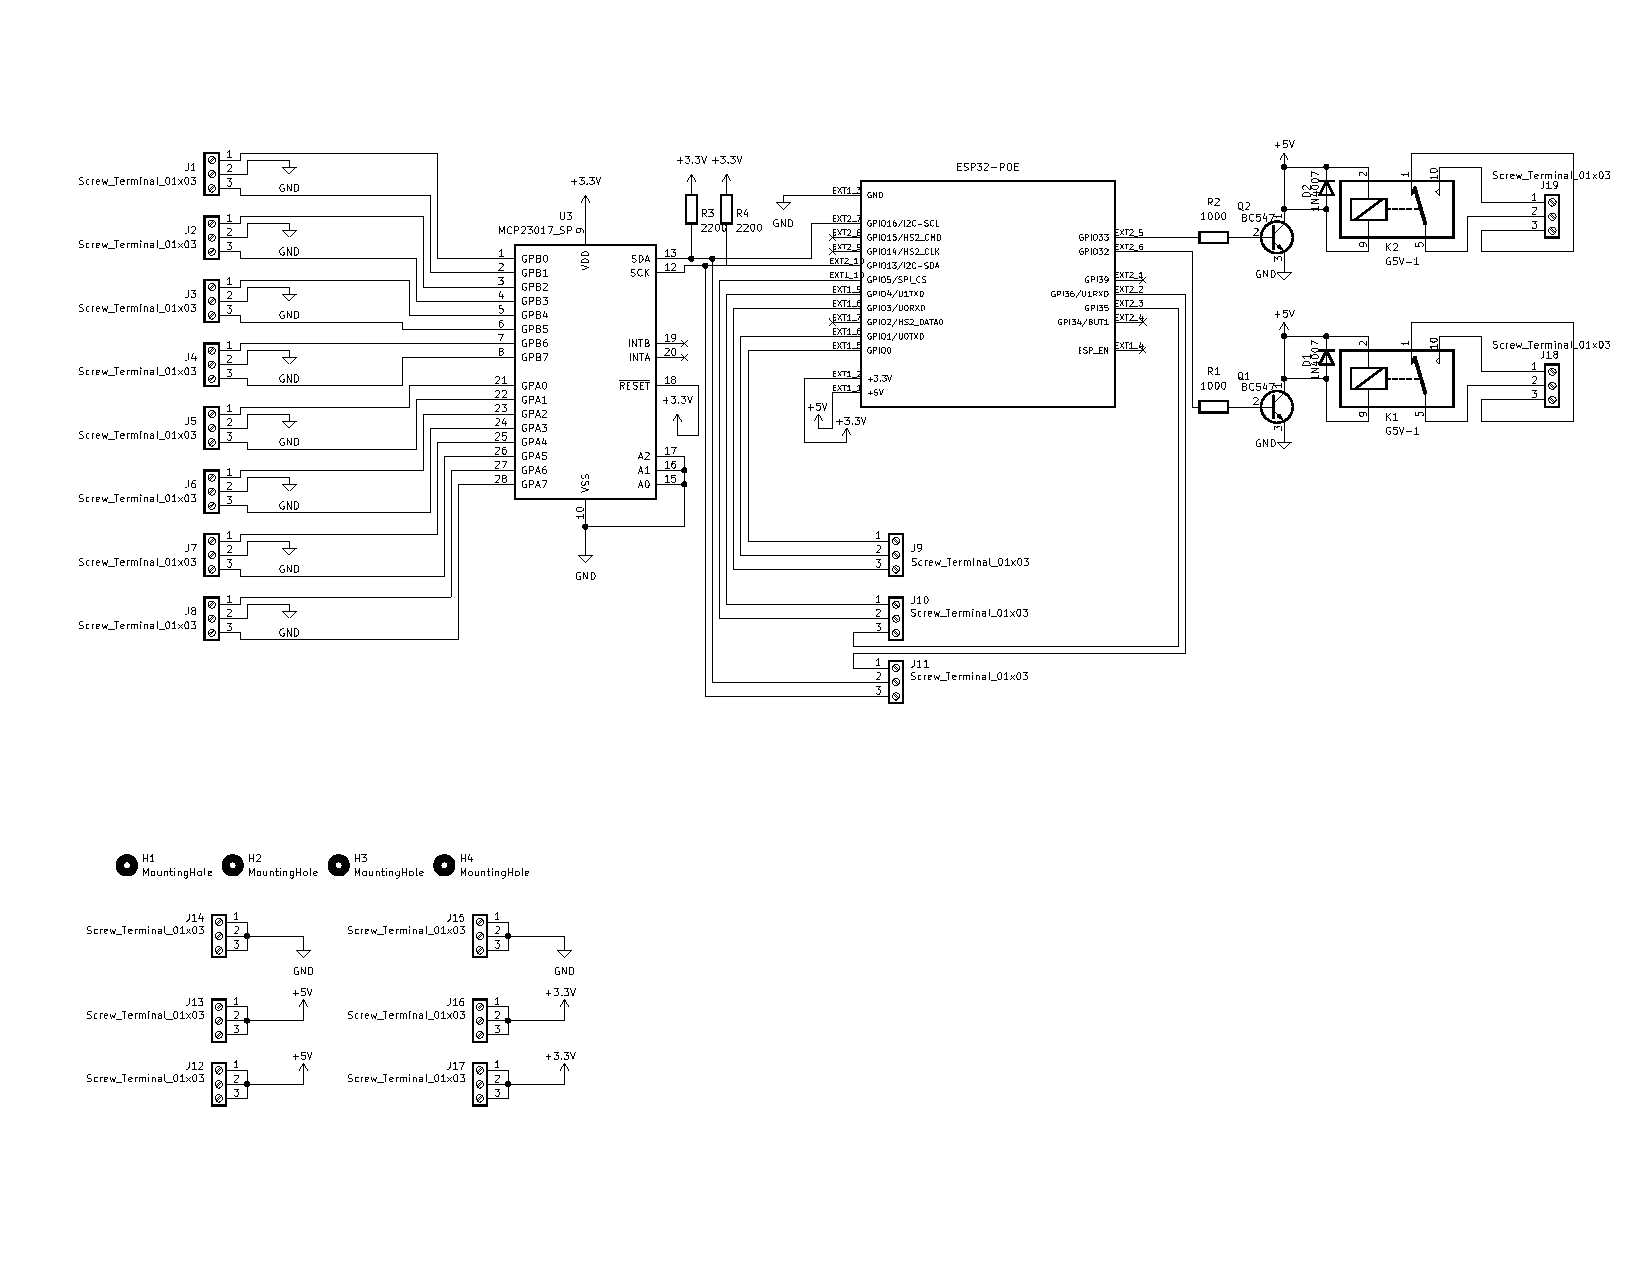
\includegraphics[width=\textwidth]{Media/Schematic.pdf}
    \caption{Schematic of the ESP32 PoE Alarm Board}
    \label{fig:schematic}
\end{figure}

\subsection{Component Selection, BOM}
The components used in the design were selected based on their availability and compatibility with the project requirements. The complete Bill of Materials (BOM), for each board, includes:

\begin{itemize}
    \item n.1 Olimex ESP32-POE development board
    \item n.1 Microchip MCP23017 GPIO expander
    \item n.2 Omron G5V-1-DC5 relays
    \item n.2 2n2222 NPN transistors
    \item n.2 1N4007 diodes
    \item n.2 2.2k$\Omega$ resistors (for I\textsuperscript{2}C pull-ups)
    \item n.2 1k$\Omega$ resistors (for transistor base)
    \item n.1 DIP 28 pin socket (for the GPIO expander)
    \item n.2 female 2.54mm 10 pin sockets (for the ESP32)
    \item n.19 5.0mm 3 pin screw terminals
\end{itemize}


\subsection{Breadboard Prototyping}
Before creating the PCB, a breadboard prototype was built to test the design and functionality of the board. The breadboard prototype included all the main components, including the ESP32 microcontroller, GPIO expander, relays, and some of the screw terminals. The prototype was used to test the validity of the schematic design, the functionality of the components, and the capabilities of the integrated LDO regulator to power the board.

The breadboard prototype was also used to test the ESPHome configuration and the integration with Home Assistant. The GPIO expander was successfully configured, and the relays were tested to ensure they could be activated and deactivated correctly. The sensors were also connected to the board, and their state changes were monitored in Home Assistant.

Once the breadboard prototype was tested and validated, the design was ready for the PCB layout.

The following image shows the breadboard prototype of the board:
\begin{figure}[H]
    \centering
    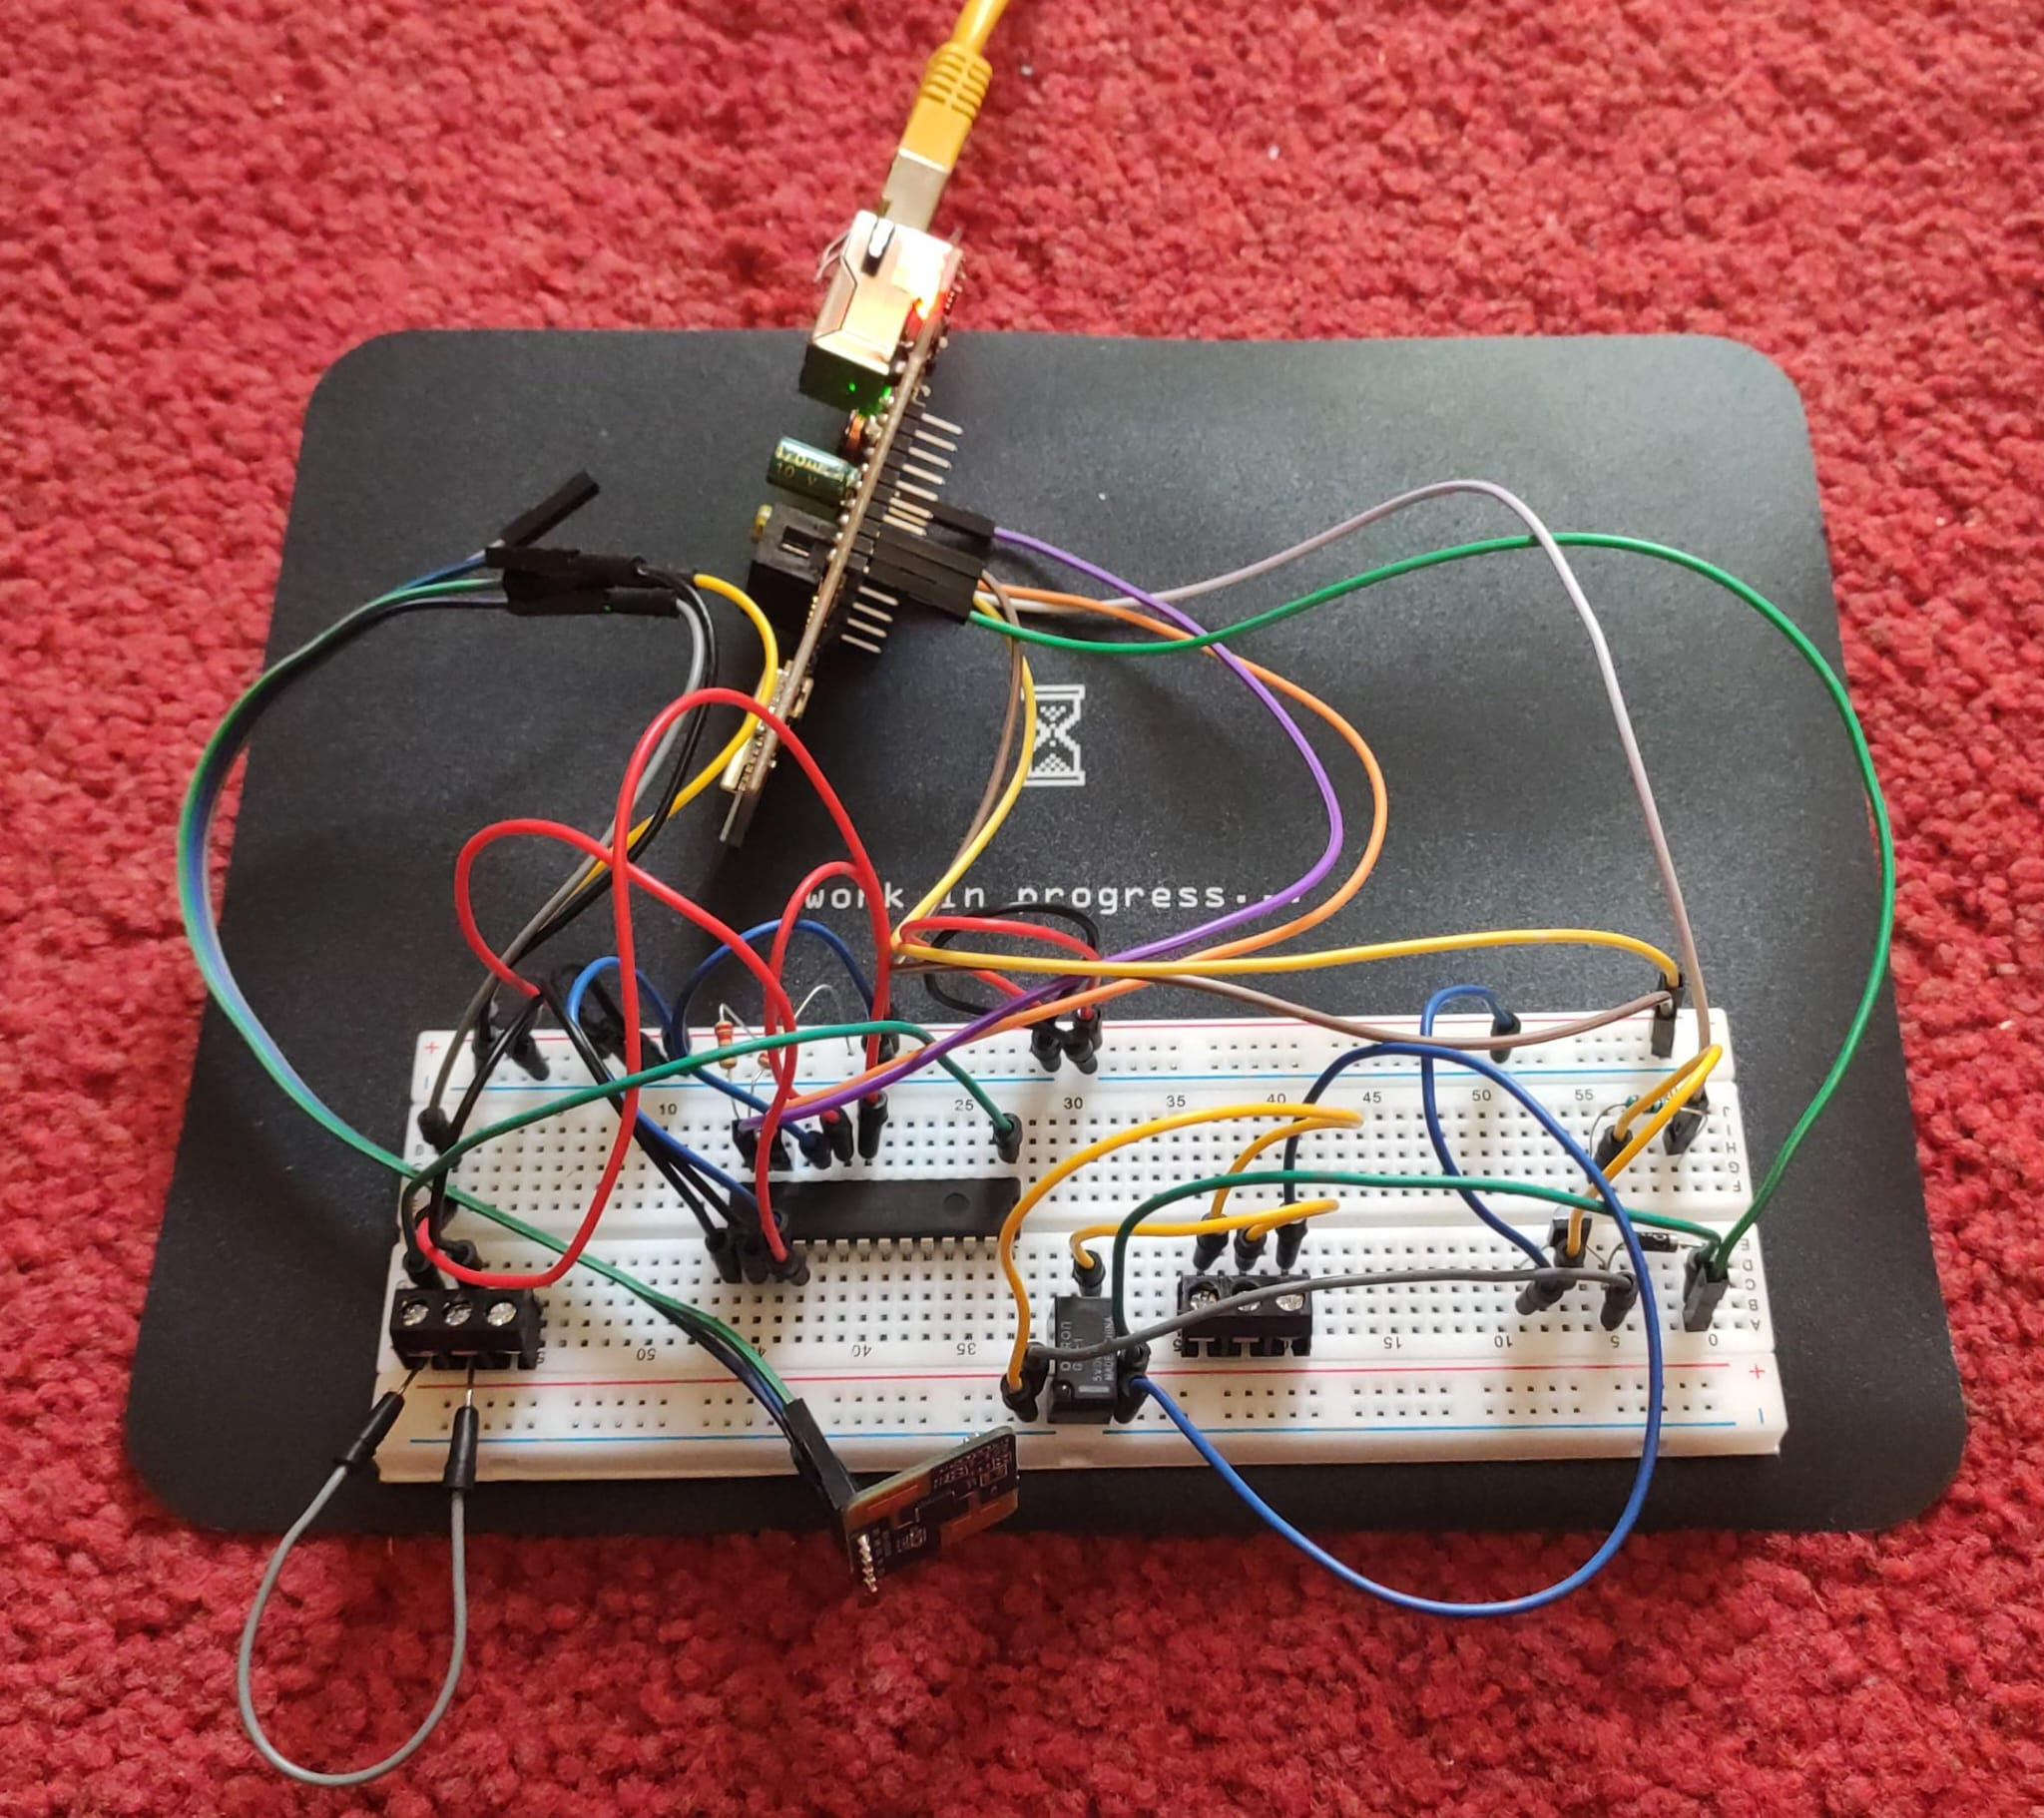
\includegraphics[width=0.8\textwidth]{Media/Breadboard.jpg}
    \caption{Breadboard prototype of the ESP32 PoE Alarm Board}
    \label{fig:breadboard}
\end{figure}

\subsection{PCB Layout}

The PCB layout was created using KiCAD, following the schematic design. The layout includes all components, traces, and pads for soldering. The board was designed to be easy to assemble, to mount, to connect to the sensors and devices, to diagnose and repair.
Because of the last point, the board wasn't targeted to be as small as possible, but rather to have all the screw mounts for the sensors on the same side of the board. The other screw terminals are grouped by functionality on the other sides of the board.

All the used components are THD, which makes the soldering process easier and faster, given the low quantity of pieces to be produced. The GPIO expander and the ESP32 are mounted using sockets, which allows for easy replacement in case of failure. This also allow the ESP32 antenna to be further away from the board itself, which improves the signal quality, in case the board were to be used with Wi-Fi connectivity instead of Ethernet, or if ESP32 Bluetooth capabilities were to be exploited.

It was possible to fit all the traces and pads on a two-layer PCB, which was a requirement for the project to be cost-effective. 

The following image shows the PCB layout, with front side traces in red and back side traces in blue. 
\begin{figure}[H]
    \centering
    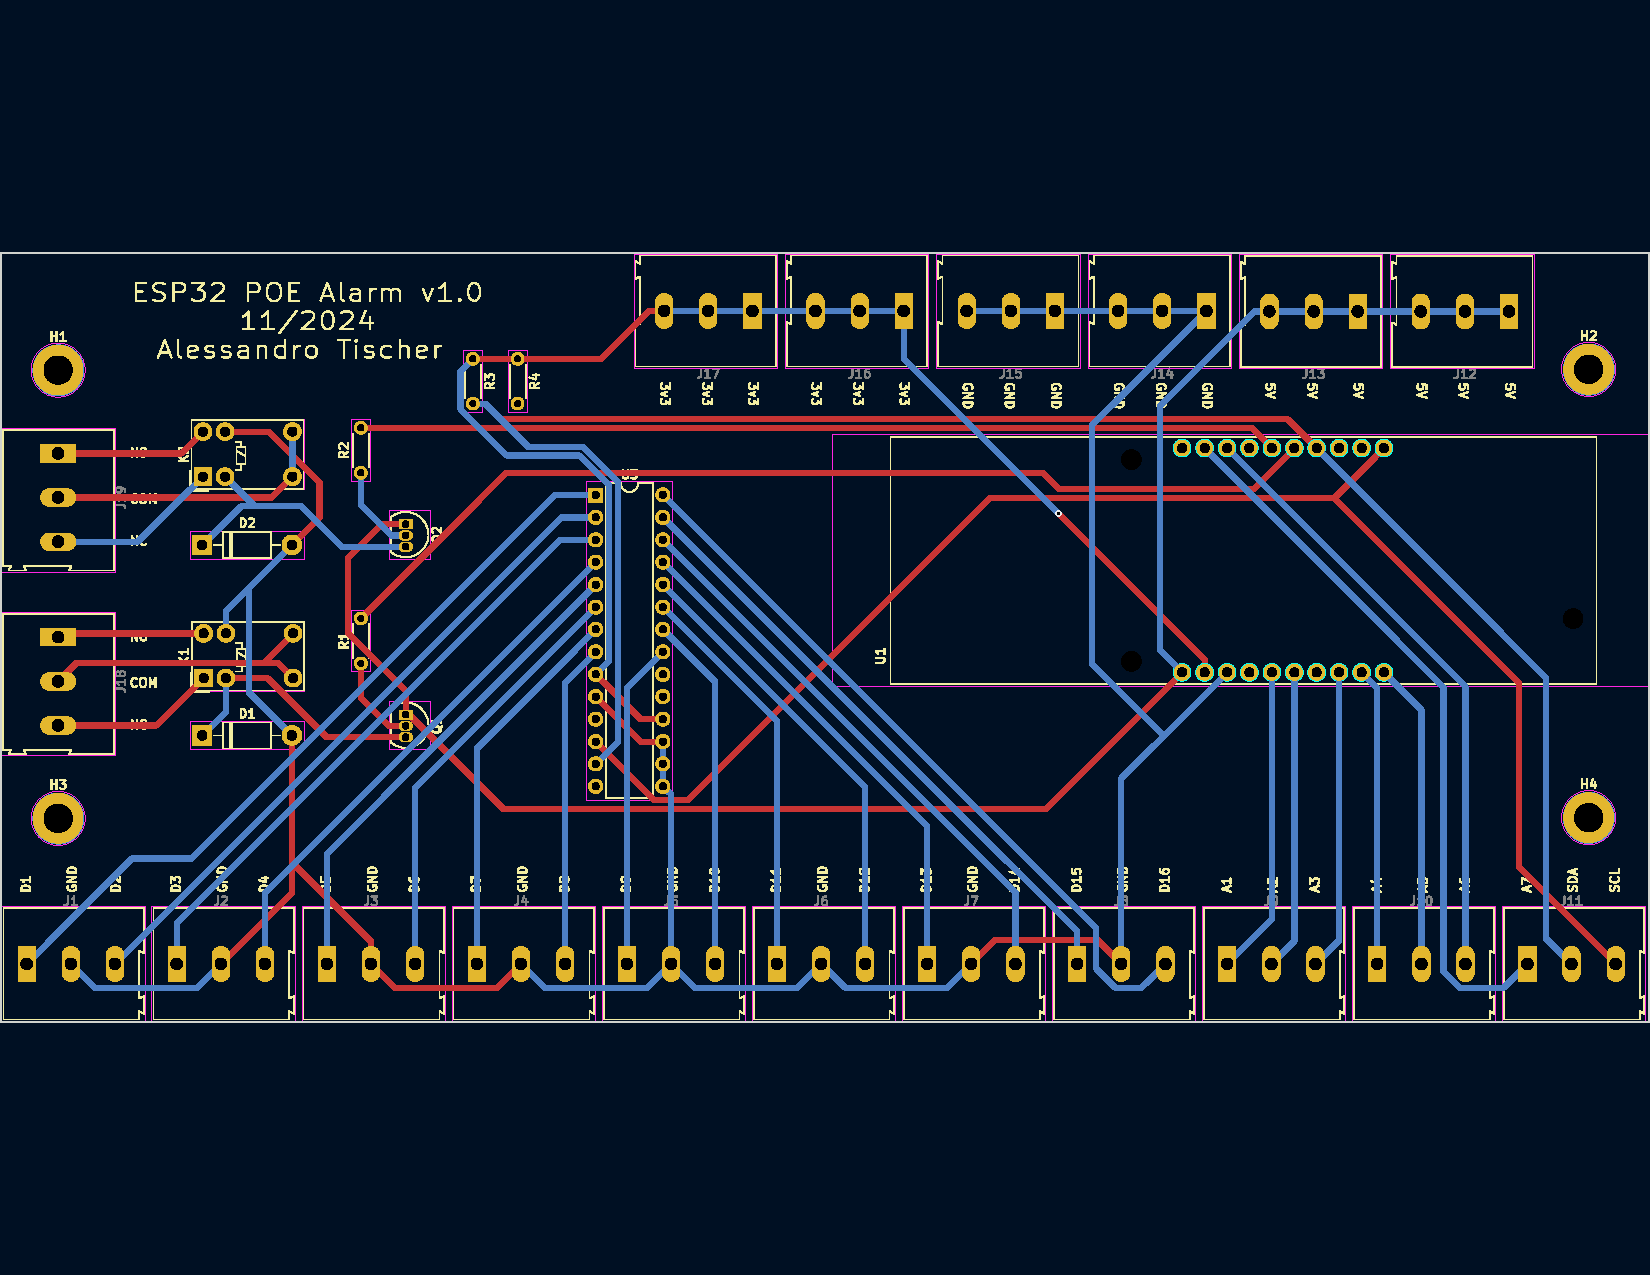
\includegraphics[width=\textwidth]{Media/PCB.pdf}
    \caption{PCB layout of the ESP32 PoE Alarm Board}
    \label{fig:pcb}
\end{figure}

\subsection{PCB Manufacturing}

The PCB was designed to be manufactured using a low-cost PCB manufacturer, which allows for easy, fast and affordable production of the board and fast shipping \cite{PCBPrototypePCB}.

In KiCAD it is possible to generate the Gerber files needed for the PCB manufacturing, which include all the necessary information for the manufacturer to produce the board. The Gerber files were generated and sent to the manufacturer.

After a few days, the PCBs were received and inspected for any defects. The boards were found to be well manufactured, with no visible defects or issues, so the assembly process could begin.

The following image shows the manufactured PCB:
\begin{figure}[H]
    \centering
    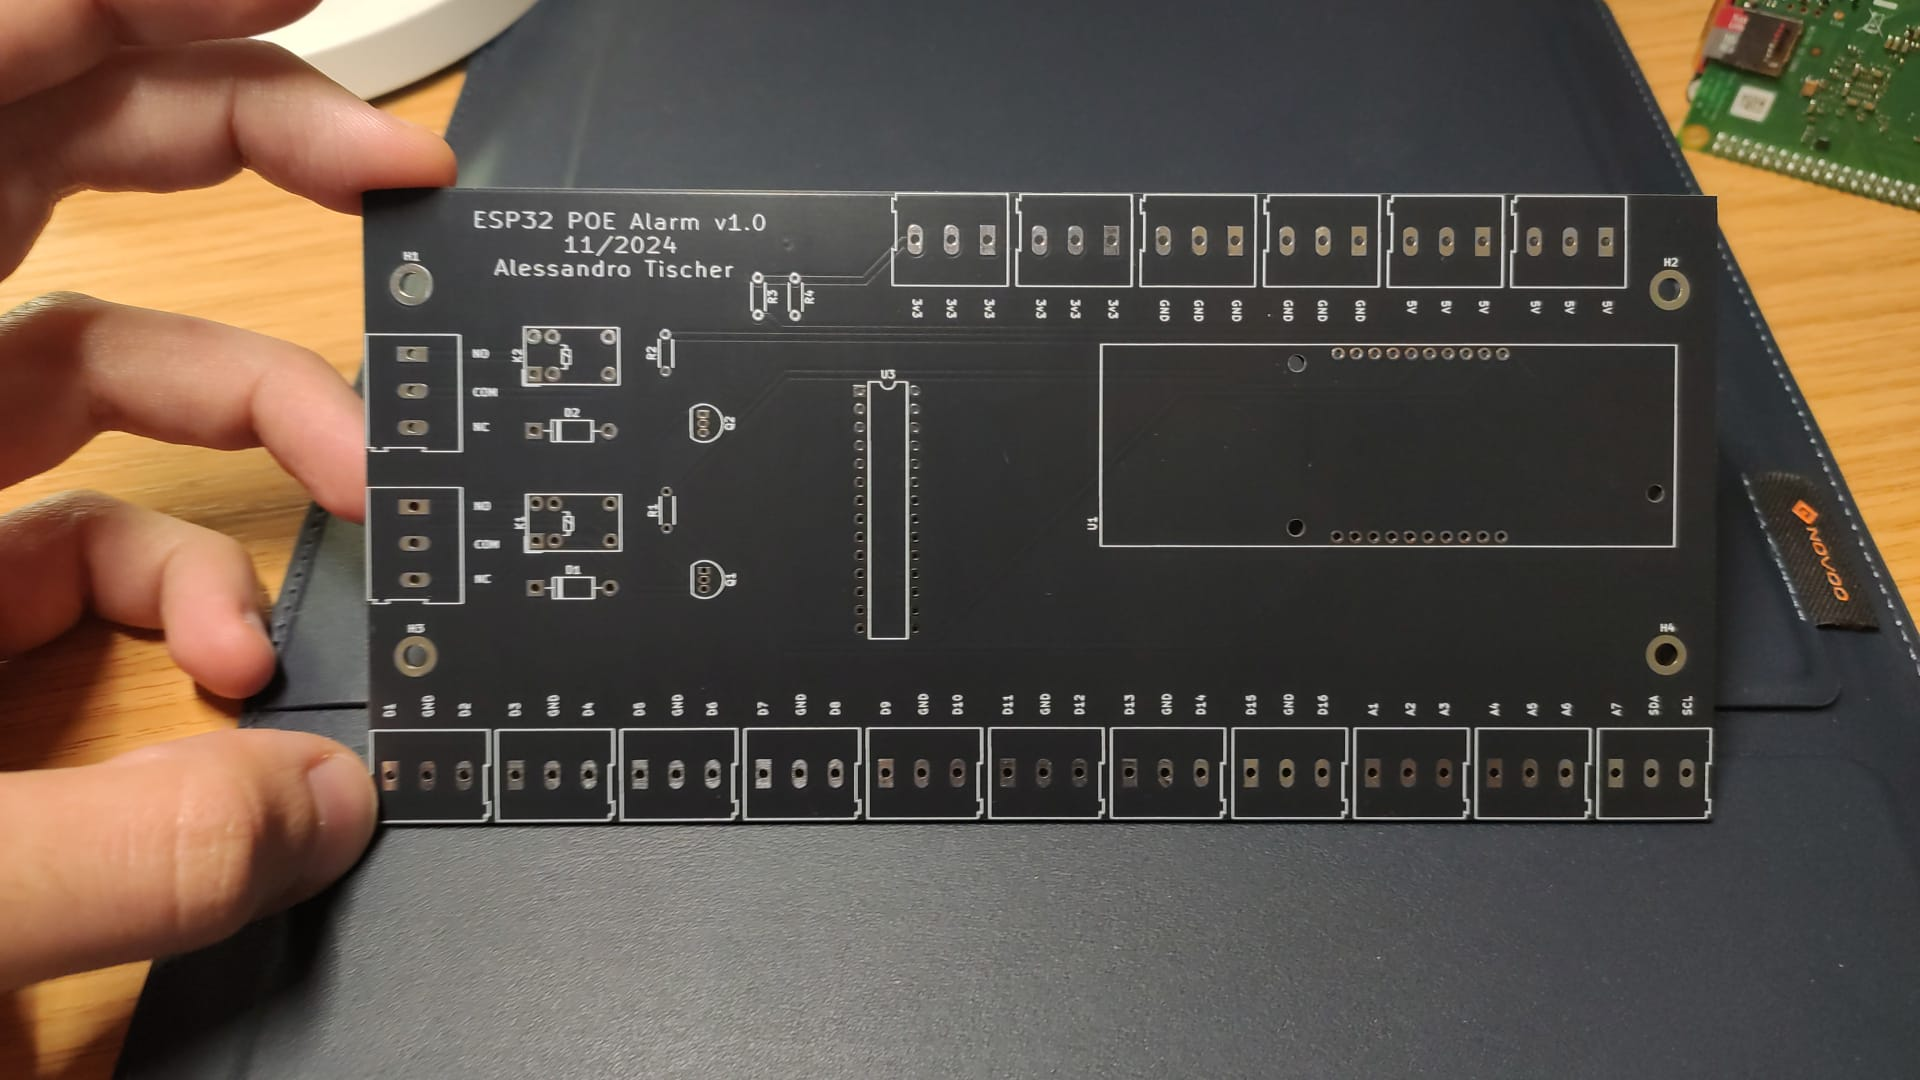
\includegraphics[width=0.8\textwidth]{Media/PCB_Manufactured.jpg}
    \caption{Manufactured PCB of the ESP32 PoE Alarm Board}
    \label{fig:manufactured_pcb}
\end{figure}

\subsection{PCB Assembly}

The assembly process was done by hand, using a soldering iron and soldering wire. The components were soldered to the PCB according to the layout, starting with the smallest components and working up to the largest ones. 

Three boards were completely assembled: two for the final application, and one to be kept as a spare in case of failure.
The assembly process was straightforward, but required quite a bit of time and patience, to avoid shorts or cold solder joints.

The following image shows the assembled PCB:
\begin{figure}[H]
    \centering
    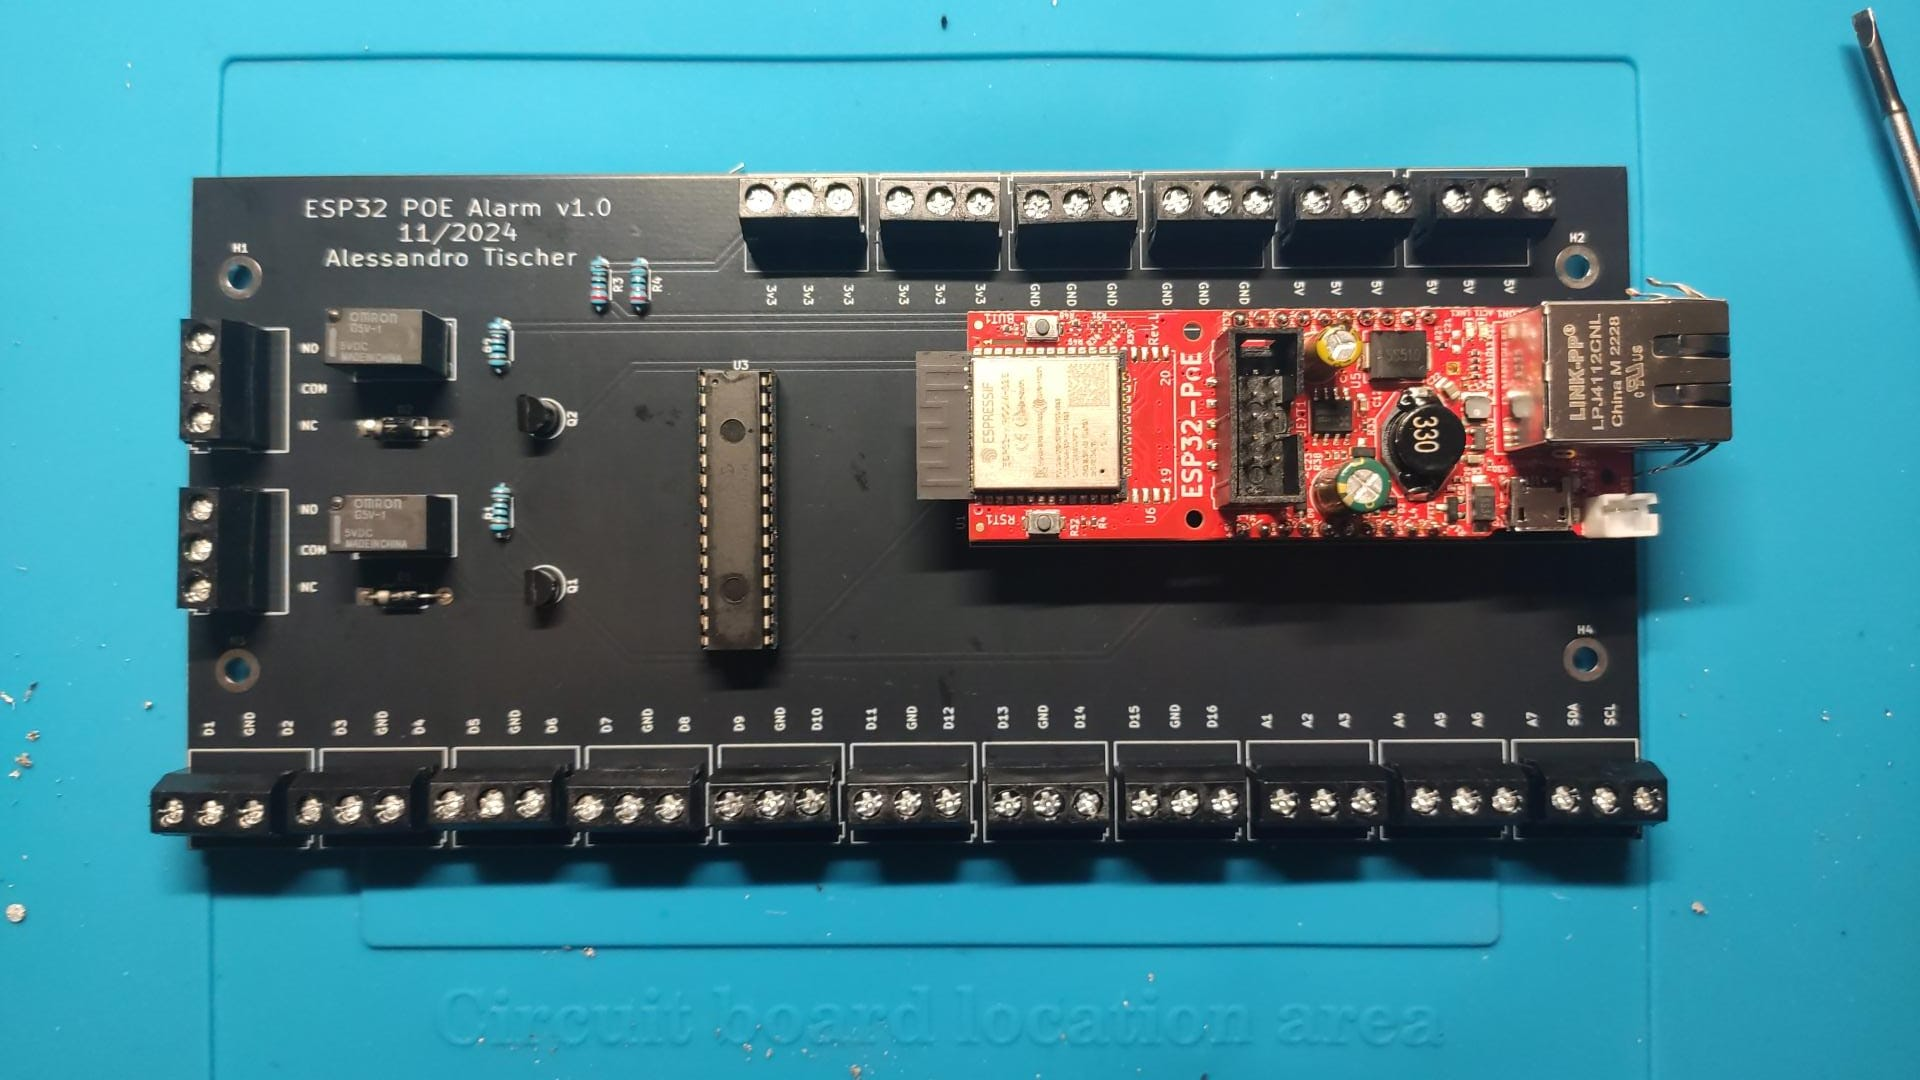
\includegraphics[width=0.8\textwidth]{Media/PCB_Assembly.jpg}
    \caption{Assembled PCB of the ESP32 PoE Alarm Board}
    \label{fig:assembled_pcb}
\end{figure}

\newpage
\section{Testing and Validation}

The first testing phase on the complete boards was done to verify the correct operation of the components and the overall functionality of the board. The tests included:

\begin{itemize}
    \item \textbf{Power supply tests:} verifying that the board powers up correctly and that the voltage levels are within the specified range across all the board.
    \item \textbf{Ethernet tests:} verifying that the Ethernet connection is working correctly.
    \item \textbf{Web UI tests:} checking that the web interface is accessible and functional.
    \item \textbf{GPIO tests:} checking that the GPIO expander is communicating with the ESP32.
    \item \textbf{Relay tests:} verifying that the relays can be activated and deactivated correctly.
    \item \textbf{Sensor tests:} checking that the GPIOs could detect a short circuit to ground.
\end{itemize}

The second testing phase was designed to verify that all initial requirements, as defined in Section~\ref{sec:MainObjectives}, were met. Each test corresponds to a specific objective or feature of the board:

\begin{itemize}
    \item \textbf{Reliable detection of state changes:} The board was tested with various digital sensors (reed switches, radar sensors, PIR sensors) to ensure prompt and accurate detection of input changes.
    \item \textbf{Low latency:} The response time between a sensor state change and the corresponding update in Home Assistant is so short that it can barely be perceived, meeting the requirement for low latency.
    \item \textbf{Integration with Home Assistant:} The board was integrated with Home Assistant, and bidirectional communication (state updates and commands) was verified.
    \item \textbf{Reliability and continuous operation:} The board was operated continuously for several days, powered via PoE and connected to a UPS, without any failures or missed events.
    \item \textbf{Ease of installation and expansion:} The modular design, use of screw terminals, and I\textsuperscript{2}C expandability were validated during assembly and sensor connection.
    \item \textbf{Data security and privacy:} Using ESPHome and Home Assistant, the board was configured to operate locally without external cloud services, ensuring intrinsic data security and privacy.
\end{itemize}

All tests were successful, confirming that the ESP32 PoE Alarm Board meets the project's objectives and requirements.

\newpage
\section{Enclosure}
The board was designed to be mounted in a plastic enclosure, which provides physical protection. The enclosure was designed in Autodesk Fusion \cite{AutodeskFusion3D} to be compact and easy to mount, with enough space for the board and the connectors. The enclosure has cutouts for the Ethernet port and the screw terminals, allowing for easy access to the connectors. The enclosure also has mounting holes for securing the board in place.
The enclosure was designed from the beginning keeping in mind that it had to be produced with additive manufacturing using a 3D printer and PLA filament. 
The enclosure was printed in two parts, which were then clicked together to form a complete enclosure. 

The following images show the 3D printed enclosures:
\begin{figure}[H]
    \subfloat{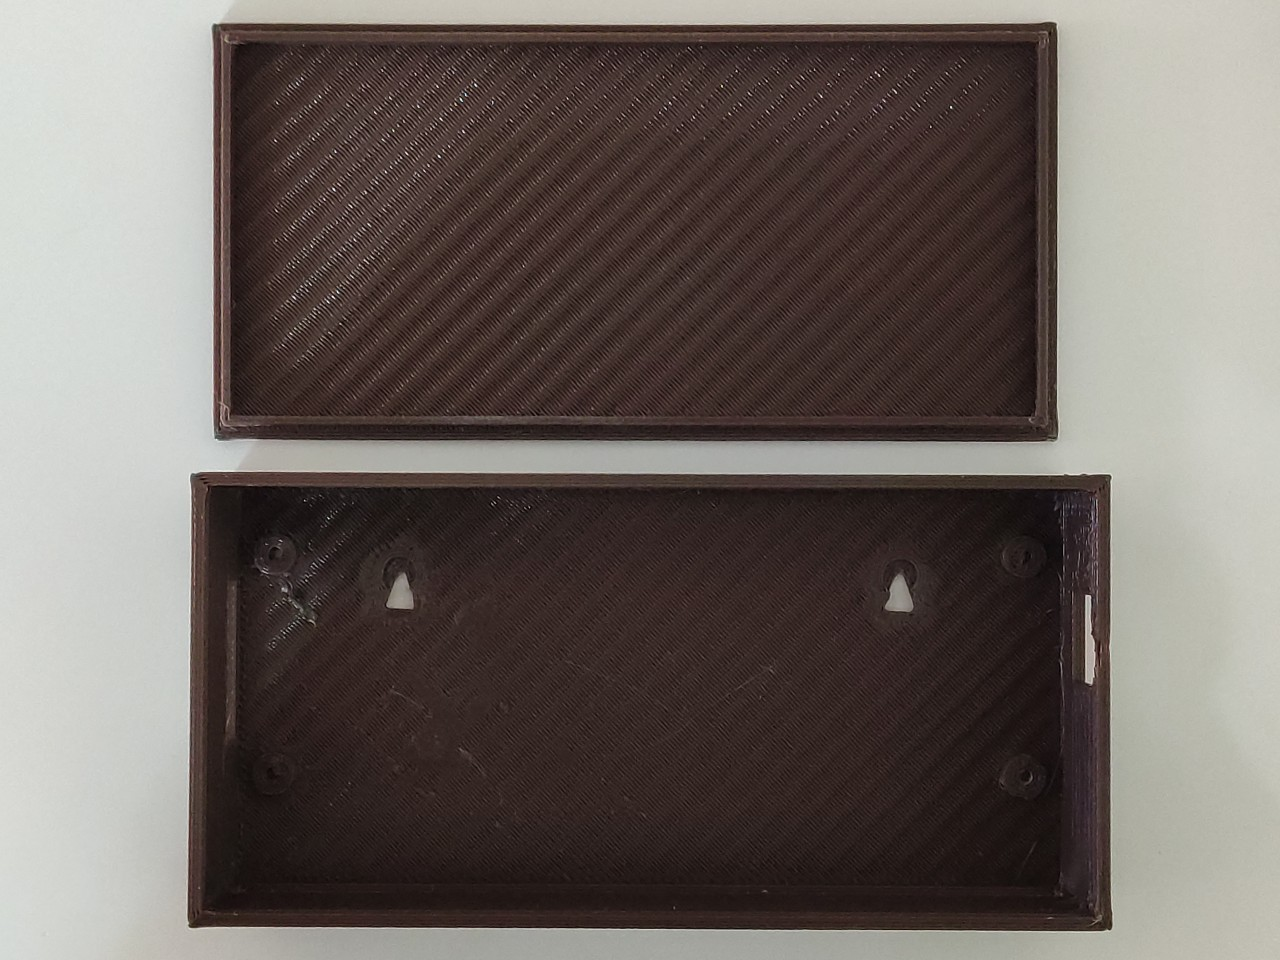
\includegraphics[width=0.48\textwidth]{Media/Enclosure.jpg}}\qquad
    \subfloat{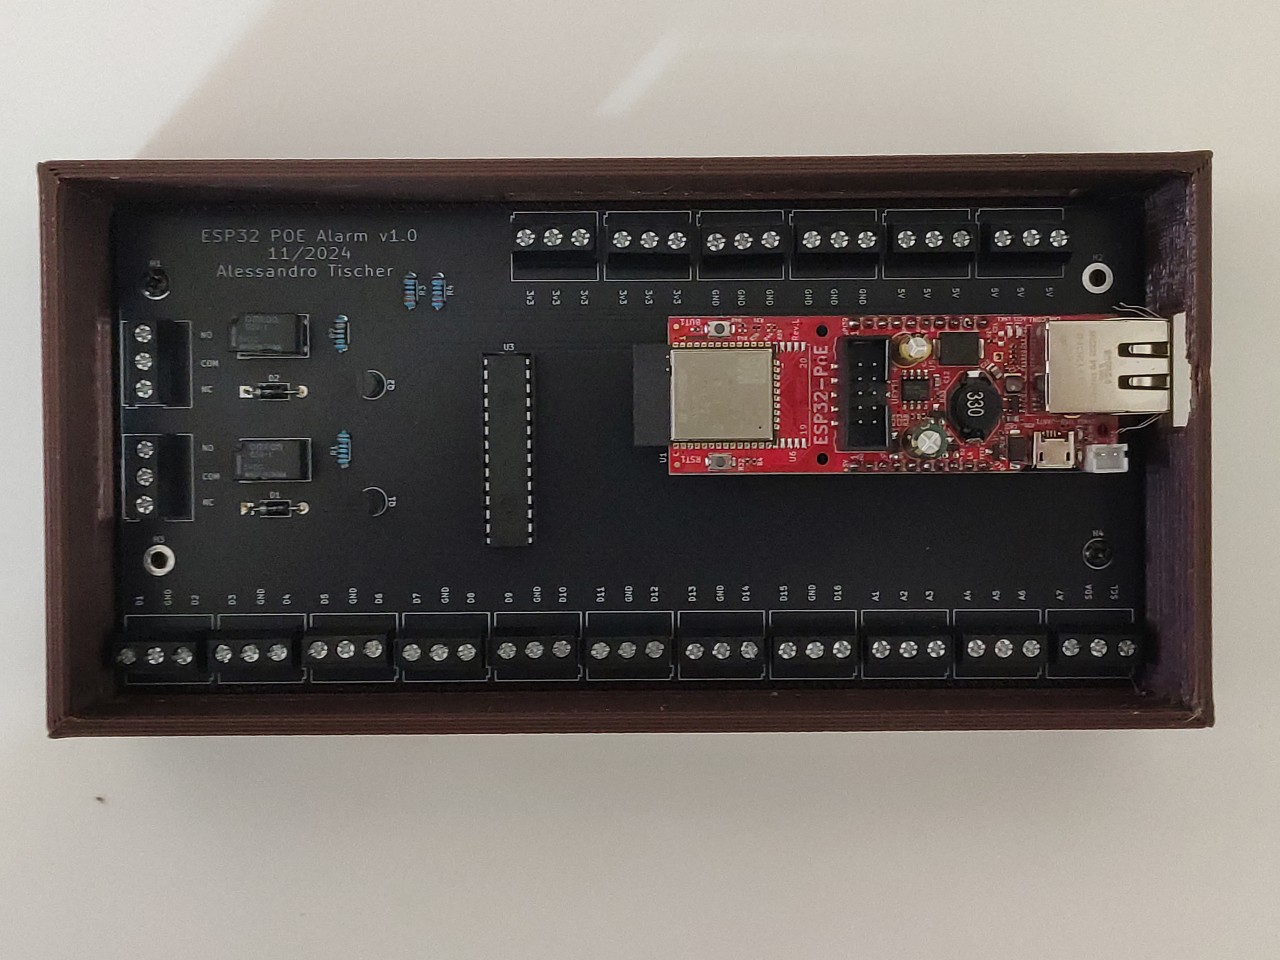
\includegraphics[width=0.48\textwidth]{Media/Enclosure1.jpg}}\\
    \subfloat{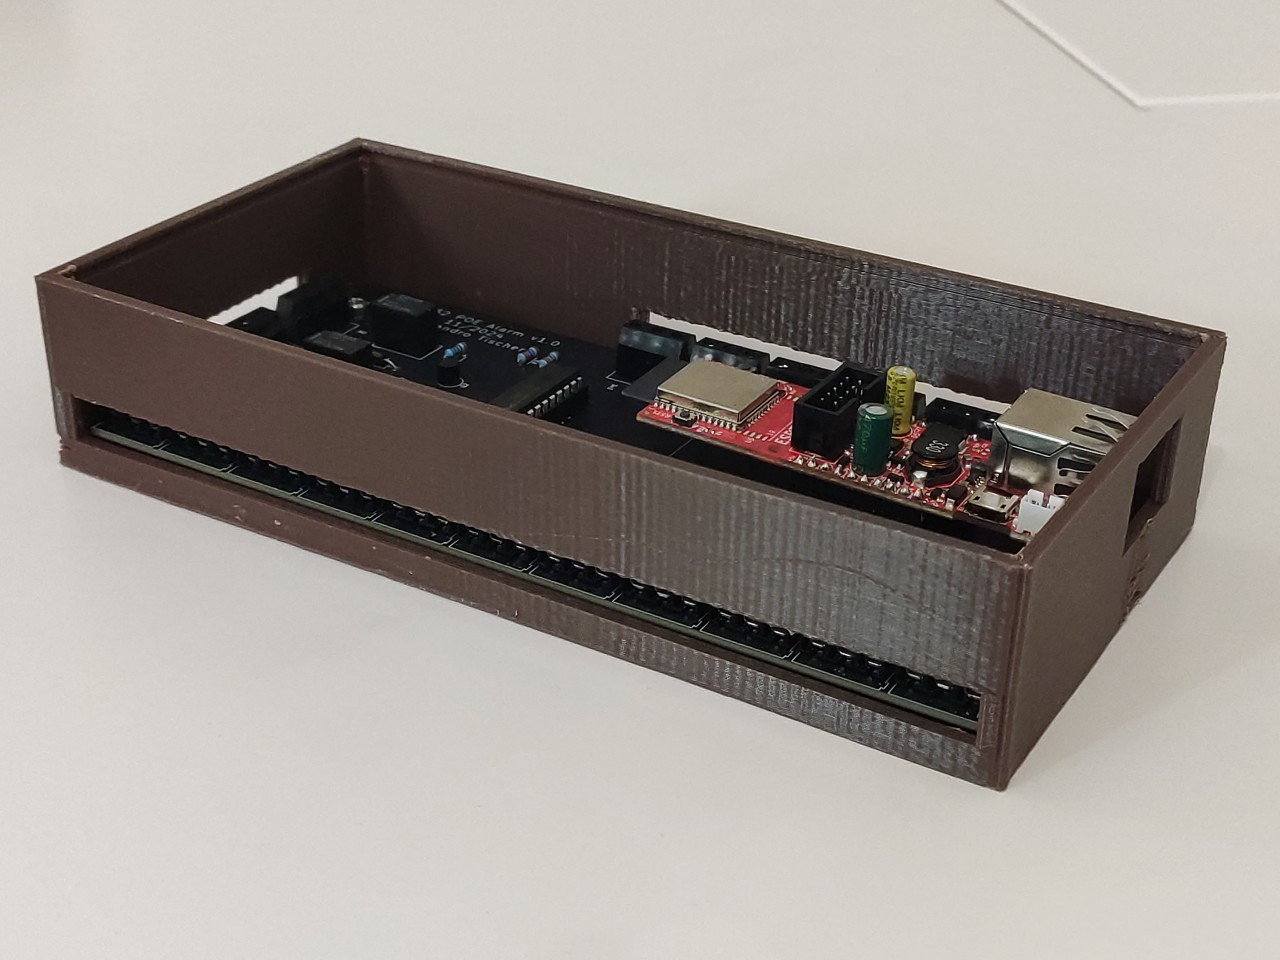
\includegraphics[width=0.48\textwidth]{Media/Enclosure2.jpg}}\qquad
    \subfloat{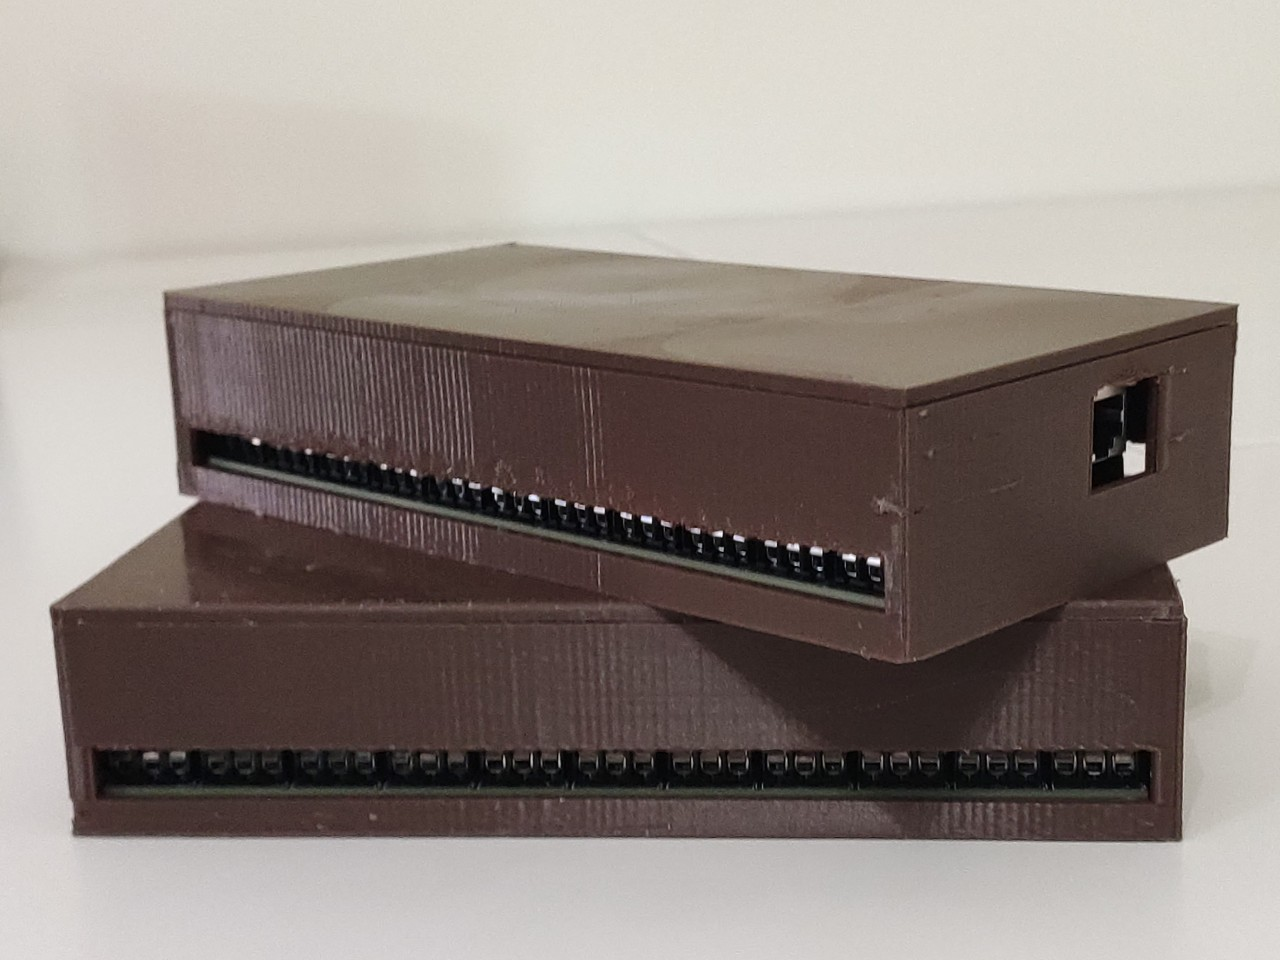
\includegraphics[width=0.48\textwidth]{Media/Enclosure3.jpg}}
    \caption{Enclosure of the ESP32 PoE Alarm Board}
    \label{fig:enclosure}
\end{figure}

\newpage
\section{Conclusion}

\subsection{Possible Improvements}
The current design of the ESP32 PoE Alarm Board is functional and meets the initial objectives. However, there are several potential improvements and enhancements that could be made in future iterations:
\begin{itemize}
    \item \textbf{Local Alarm Logic}: Implementing local alarm logic on the board could provide additional functionality and reduce reliance on Home Assistant for alarm management.
    \item \textbf{Integrated ESP32 Module}: Using an integrated ESP32 module instead of a development board could reduce the size and cost of the board, while also improving customization options. For example, designing a custom PoE module, would allow having more power budget for the board.
    \item \textbf{Short Bypass Detection}: In professional alarm systems, a small resistor is connected in series with the reed switch, just before the sensor itself. This resistor is used to detect if the sensor is bypassed by a short circuit made to tamper with the system. Monitoring the resistance on the wire allows detecting if the sensor is bypassed, and to trigger an alarm. This feature was not implemented as the GPIO expander's pins are not connected to an ADC, so it would be impossible to monitor the resistance. In order to keep both the circuit and the software as simple as possible, the GPIO expander was used instead of a more complex solution that would allow monitoring the resistance. However, this feature could be added in the future by using an analog multiplexer or a diode matrix instead of the GPIO expander if the application requires more security.
\end{itemize}

\subsection{Lessons Learned}
The project provided valuable insights into the design and development of a custom PoE alarm system. Key lessons learned include:
\begin{itemize}
    \item The importance of thorough research and component selection to ensure compatibility and functionality.
    \item The benefits of using open-source platforms.
    \item The value of prototyping and testing to validate designs before finalizing the PCB layout.
    \item The significance of clear documentation and organization in the design process to facilitate future modifications and enhancements.
    \item The need for careful consideration of power supply requirements and the impact of component choices on overall system performance.
    \item The importance of designing for ease of assembly and maintenance, including the use of sockets for critical components.
    \item The benefits of using modular designs to allow for future expansion and customization.
    \item The value of testing and validation to ensure the final product meets the initial objectives and requirements.
\end{itemize}

\subsection{Final Remarks}
This project was challenging but rewarding, as it involved researching and learning about various components, software, and design techniques. Particularly demanding were the phases of definition of the requirements, finding and reading the datasheets of the components and checking their compatibility with each other, as well as the design of the schematic and PCB. 

The final product reflects the initial objectives and requirements, providing a reliable and flexible solution for the PoE alarm system. The board is capable of monitoring multiple sensors, controlling devices, and integrating with Home Assistant, making it a valuable addition to any home automation system.

\newpage
\bibliographystyle{unsrturl}
\bibliography{References/Esp32PoEAlarm.bib}


\end{document}